% Bekannte Fehler
\section{Bekannte Fehler}

\subsection{iOS6 - Add to homescreen}
Eine sehr nützliche Funktionalität, welche Apple im Mobile Safari-Browser anbietet ist die \emph{Add to homescreen}-Funktion.

\begin{figure}[H]
\subfigure{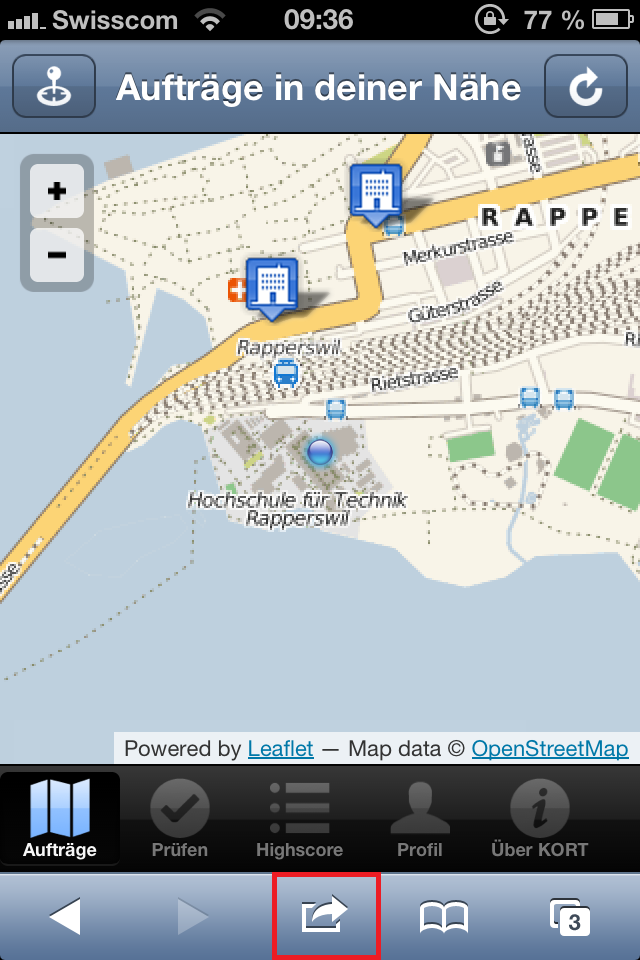
\includegraphics[width=0.23\textwidth]{images/bugs/kort-add_to_homescreen_1}}
\hfill
\subfigure{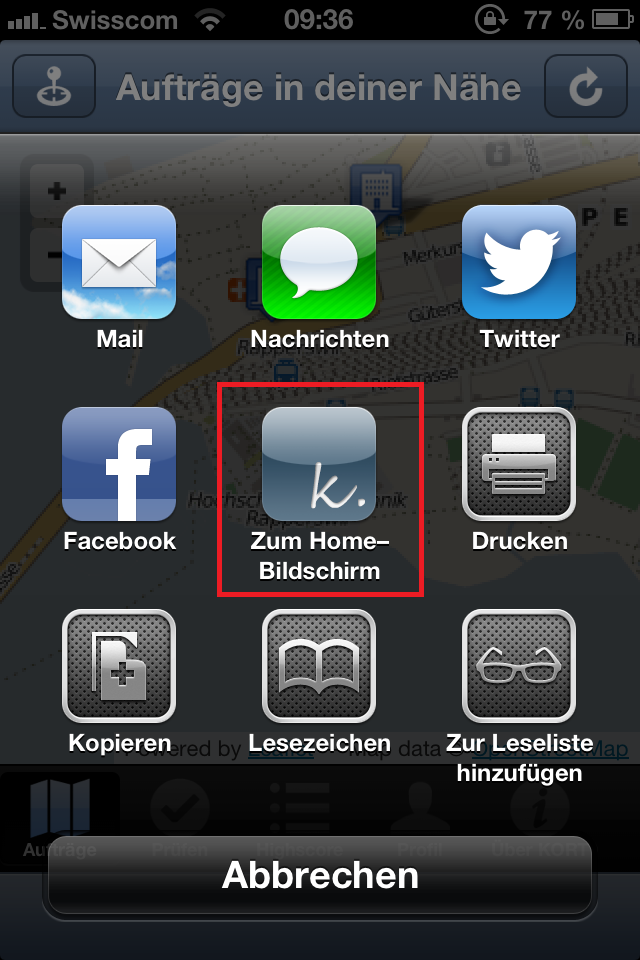
\includegraphics[width=0.23\textwidth]{images/bugs/kort-add_to_homescreen_2}}
\hfill
\subfigure{
\includegraphics[width=0.23\textwidth]{images/bugs/kort-add_to_homescreen_3}}
\hfill
\subfigure{
\includegraphics[width=0.23\textwidth]{images/bugs/kort-add_to_homescreen_4}}
\caption{iOS - "`Add to homescreen"'-Funktion}
\end{figure}

Dadurch wird ein App-ähnlicher Bookmark der aktuellen Webseite auf dem Homescreen erstellt.
Dieser erhält ein hinterlegtes Icon und einen Titel.
Beim Starten der App erscheint ein Splashscreen, welchen man ebenfalls in der Webseite definieren kann.
Zudem öffnet sich der Browser ohne jegliche Toolbars wie der Adress- oder der Navigationsleiste.

Leider befindet in iOS6 ein Bug, welcher den Zugriff auf die Geolocation verhindert, wenn die \gls{WebApp} vom Homescreen aus gestartet wird.
Auf Stack Overflow\footnote{\url{http://stackoverflow.com/questions/12503815/ios-6-breaks-geolocation-in-webapps-apple-mobile-web-app-capable}} wird der Bug genauer beschrieben.

\textbf{Workaround}

Im Sencha Fourm\footnote{\url{http://www.sencha.com/forum/showthread.php?246317-2.1.0-RC1-Save-to-home-screen-Geolocation-not-working}} wird als Workaround vorgeschlagen die Generierung des folgenden Metatags (siehe Code-Ausschnitt \ref{code-ios6-homescreen-metatag}) in der Sencha Touch Library zu deaktivieren.

\lstset{language=HTML}
\begin{lstlisting}[caption=Metatag für iOS6 Workaround, label=code-ios6-homescreen-metatag]
<meta content="yes" name="apple-mobile-web-app-capable" />
\end{lstlisting}

Diese befindet sich in folgenden Dateien:

\begin{itemize}
\item \inlinecode{/touch/microloader/development.js} Zeile 24
\item \inlinecode{/touch/microloader/production.js} Zeile 564
\item \inlinecode{/touch/microloader/testing.js} Zeile 24
\item \inlinecode{/touch/sencha-touch-all-debug.js} Zeile 9345
\item \inlinecode{/touch/sencha-touch-debug.js} Zeile 9345
\item \inlinecode{/touch/src/core/Ext-more.js} Zeile 657
\end{itemize}

Das Deaktivieren dieser Zeile hat aber zur Folge, dass der native Rahmen des Browsers (Adressleiste, Navigationsleiste) wieder angezeigt wird.
Dies ist zwar unschön löst aber das Problem mit dem Zugriff auf die Geolocation.

\subsection{App Build}
Wie in Abschnitt \ref{sencha-cmd} beschrieben, basiert die App vollständig auf dem Sencha-eigenen Build-Tool \brand{Sencha Cmd 3.0.0.250}. Darin sind aber noch einige Bugs vorhanden.

Bei \kort{} besteht dabei ein Problem bei der fest eingebauten Komprimierung der JavaScript-Sourcen.
Während diesem Prozess werden lokale Variablennamen mit einzelnen Buchstaben abgekürzt.
Dabei treten Konflikte mit der \brand{Leaflet}-Library auf, welche den Buchstaben \emph{L} als Namespace verwendet.

\textbf{Workaround}

Um diese Problem zu umgehen, mussten wir das Build-Skript von \brand{Sencha Cmd} minimal anpassen.
So mussten wir die Zeile, welche den \gls{Microloader} komprimiert auskommentieren (siehe Code-Ausschnitt \ref{senchacmd-workaround}).
Diese befindet sich in folgender Datei:

\inlinecode{/<Sencha Cmd Verzeichnis>/plugins/touch/current/app-build.js} Zeile 362

\lstset{language=JavaScript}
\begin{lstlisting}[caption=Sencha Cmd Workaround, label=senchacmd-workaround]
processIndex = function () {
	[...]
	
	compressor = new ClosureCompressor();
	microloader = (environment == 'production'
		? 'production'
		: 'testing') +
		'.js';
	_logger.debug("using microloader : {}", microloader);
	content = readFileContent(joinPath(sdk, "microloader", microloader));
	//content = compressor.compress(content);
	remotes = [
		'<script type="text/javascript">' +
			content + ';Ext.blink(' +
			(environment == 'production' ? jsonEncode({
				id:config.id
			}) : appJson) + ')' +
			'</script>'
	];
	
	[...]
};
\end{lstlisting}